\section{Discussion}\label{sec:chp3:dis}


\subsection{Results reported}\label{subsec:chp3:dis:res}

As discussed previously in \ac{sec}\,\ref{subsec:chp3:img-clas:eval-mea}, different metrics have been used to report results.
A comparison of the different methods reviewed is given depending on the metric used in field of research and also the type of \ac{mri} scanner used, i.e. \SI{1.5}{\tesla} or \SI{3}{\tesla}.
For each field, the \textit{best classification performance} obtained in each study have been reported in these figures.
The results in terms of \ac{auc}-\ac{roc} are depicted in \acs{fig}\,\ref{fig:auc}.
The results vary from \SIrange{71}{97}{\percent} for some experiments with a \SI{1.5}{\tesla} \ac{mri} scanner and from \SIrange{77}{95}{\percent} with a \SI{3}{\tesla} \ac{mri} scanner. 

The results in regard of sensitivity and specificity are reported in \acs{fig}\,\ref{fig:sensspec}.
In the case that the data have been collected with a \SI{1.5}{\tesla} \ac{mri} scanner, the sensitivity ranges from \SIrange{74}{100}{\percent} and the specificity from \SIrange{43}{93}{\percent}.
For the experiments carried out with a \SI{3}{\tesla} \ac{mri} scanner, the sensitivity varies from \SIrange{60}{99}{\percent} and the specificity from \SIrange{66}{100}{\percent}.
Four studies also use \ac{froc} analysis to report their results and are reported in \ac{fig}\,\ref{fig:froc}.

\begin{figure}
  \centering
  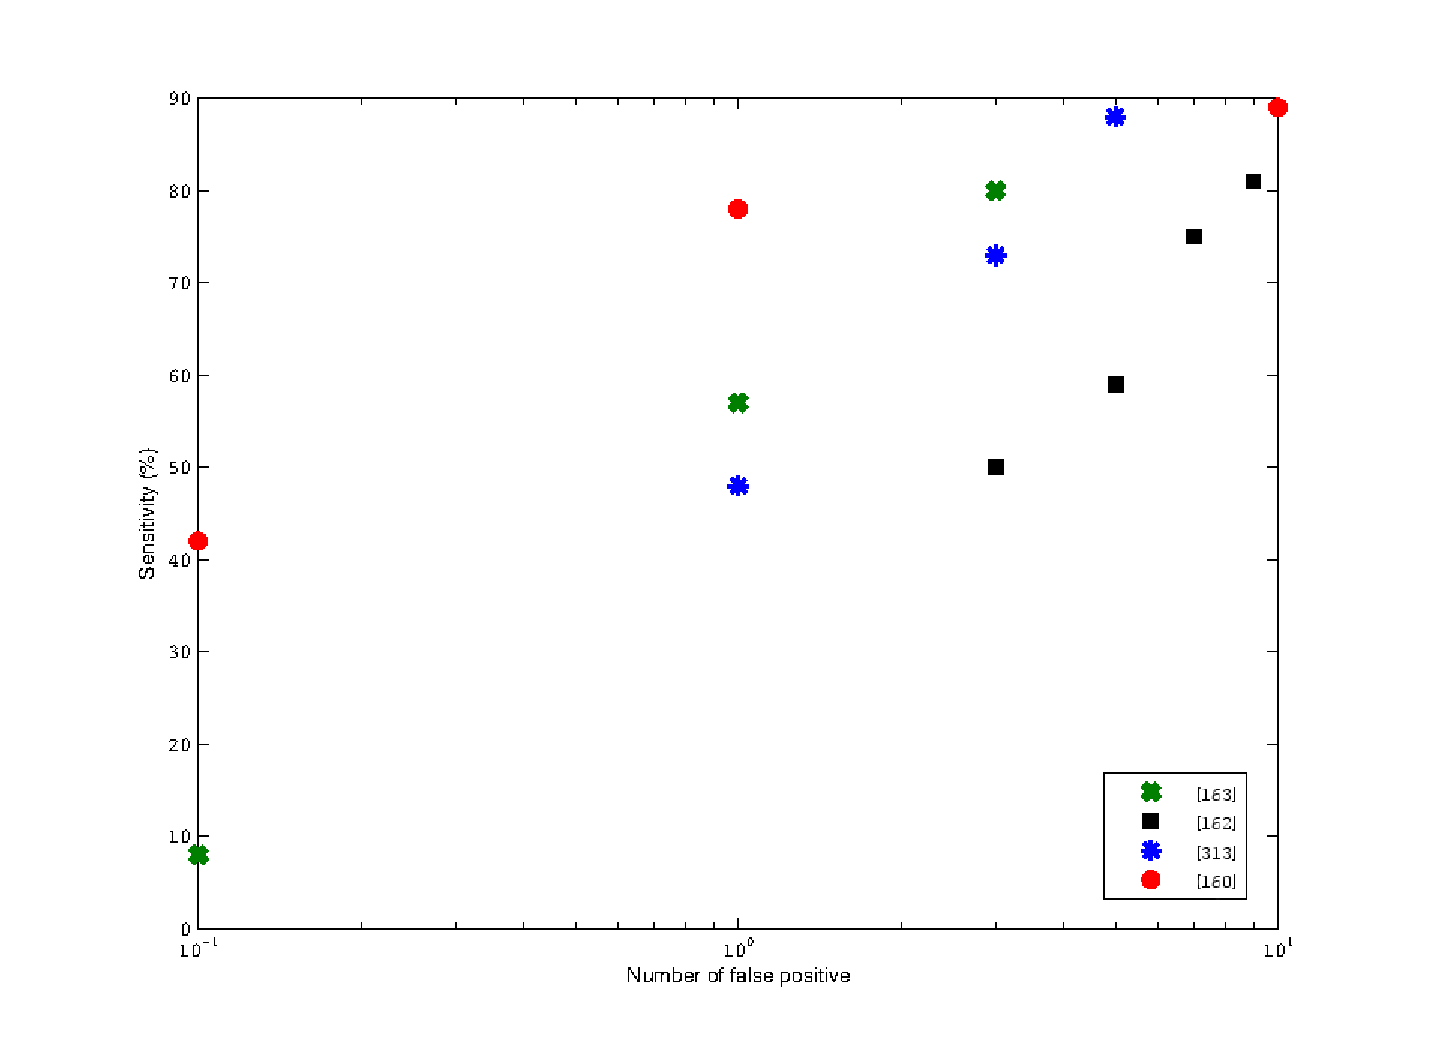
\includegraphics[width=.8\linewidth]{3_review/figures/results/froc.eps}
  \caption{Comparison in terms of \acs*{froc} of the methods using data from \SI{3}{\tesla} \acs*{mri} scanner.}
  \label{fig:froc}
\end{figure}

\begin{figure}
  \centering
 % \hspace{\fill}
  \subfigure[]{
    \label{fig:auc15}
    \begin{tikzpicture}[scale=.7,every node/.style={scale=0.7}]

      \def\labels{
        {\color{blue}\cite{Ampeliotis2008}},
        {\color{blue}\cite{Antic2013}},
        {\color{blue}\cite{Chan2003}},
        {\color{blue}\cite{Giannini2013}},
        {\color{blue}\cite{Langer2009}},
        {\color{blue}\cite{Lopes2011}},
        {\color{blue}\cite{Lv2009}},
        {\color{blue}\cite{Niaf2011}},
        {\color{blue}\cite{Niaf2012}},
        {\color{blue}\cite{Tiwari2009a}},
        {\color{blue}\cite{Tiwari2010}},
        {\color{blue}\cite{Tiwari2012}},
        {\color{blue}\cite{Tiwari2013}},
        {\color{blue}\cite{Vos2008}},
        {\color{blue}\cite{Vos2010}},
        {\color{blue}\cite{lehaire2014computer}},
        {\color{blue}\cite{giannini2015fully}},
        {\color{blue}\cite{Mazzetti2011}},
        {\color{blue}\cite{Puech2009}},
        {\color{blue}\cite{Vos2008a}},
        {\color{blue}\cite{rampun2016computerb}},
        {\color{blue}\cite{rampun2016computer}} 
      }

      \def\reward{90,94,84,87,71,93,97,87,87,84,91,90,85,91,97,75,91,92,77,90,93,93}
      \def\dbSize{25,53,15,10,25,27,55,23,30,15,19,36,29,29,29,35,56,29,100,10,45,45}
      \def\dbClass{1,2,1,1,1,1,2,1,1,1,1,1,1,1,1,1,2,1,3,1,2,2}
      \def\cZoom{3} 
      \def\percentageLabelAngle{90}
      \def\nbeams{22}
      \pgfmathsetmacro\beamAngle{(360/\nbeams)}
      \pgfmathsetmacro\halfAngle{(180/\nbeams)}
      \pgfmathsetmacro\globalRotation{\halfAngle}

      % draw the radiants
      \foreach \n  [count=\ni] in \labels
      {
        \pgfmathsetmacro\cAngle{{(\ni*(360/\nbeams))+\globalRotation}}
        \draw(\cAngle:{\cZoom*1.15})  node[fill=white] {\n};
        \draw [thin] (0,0) -- (\cAngle:{\cZoom*1}) ;

      }

      % draw the % rings 
      \foreach \x in {12.5,25, ...,100} 
      \draw [thin,color=gray!50] (0,0) circle [radius={\cZoom*\x/100}];

      \foreach \x in {50,75,100}
      { 
        \draw [thin,color=black!50] (0,0) circle [radius={\cZoom/100*\x}];
        \foreach \a in {0, 180} \draw ({\percentageLabelAngle+\a}:{\cZoom*0.01*\x}) node  [inner sep=0pt,outer sep=0pt,fill=white,font=\fontsize{8}{8.5}\selectfont]{$\x\%$};
      }

      % draw the path of the percentages
      \def\aux{{\reward}}
      \pgfmathsetmacro\origin{\aux[\nbeams-1]} 
      \draw [semiAuto, thick] (\globalRotation:{\cZoom*\origin/100}) \foreach \n  [count=\ni] in \reward { -- ({(\ni*(360/\nbeams))+\globalRotation}:{\cZoom*\n/100}) } ;

      % label all the percentags
      \foreach \n [count=\ni] in \dbSize 
      {
        \pgfmathsetmacro\cAngle{{(\ni*(360/\nbeams))+\globalRotation}}
        \pgfmathsetmacro\nreward{\aux[\ni-1]}
        \draw (\cAngle:{\cZoom*1.5}) node[align=center] {{\color{semiAuto}\nreward $\%$} \\ {\color{red}\n} };
      } ;

      % draw the database rose
      \def\dbScale{\9}
      \foreach \n [count=\ni] in \dbClass
      \filldraw[fill=red!20!white, draw=red!50!black]
      (0,0) -- ({\ni*(360/\nbeams)-\halfAngle+\globalRotation}:{\cZoom*\n/9}) arc ({\ni*(360/\nbeams)-\halfAngle+\globalRotation}:{\ni*(360/\nbeams)+\halfAngle+\globalRotation}:{\cZoom*\n/9}) -- cycle;
      \foreach \x in {1,2,3}
      \draw [thin,color=red!50!black,dashed] (0,0) circle [radius={\cZoom*\x/9}];

      %% draw the domain of each class 
      \def\puta{17/0/{Multiparametric},
        5/17/{Monoparametric}}

      \foreach \numElm/\contadorQueNoSeCalcular/\name [count=\ni] in \puta
      {

        \pgfmathsetmacro\initialAngle{(\contadorQueNoSeCalcular*\beamAngle)+\halfAngle+\globalRotation}
        \pgfmathsetmacro\finalAngle  {((\numElm+\contadorQueNoSeCalcular)*\beamAngle)+\halfAngle+\globalRotation}
        \pgfmathsetmacro\l  {\cZoom*1.65+.3pt}
        \draw (\initialAngle:{\cZoom*1.7}) -- (\initialAngle:{\cZoom*1.1});
        \draw [ |<->|,>=latex] (\initialAngle:\l) arc (\initialAngle:\finalAngle:\l) ;     
        \pgfmathsetmacro\r  {\cZoom*1.65+.45pt}
        {\draw [decoration={raise=4pt,text along path,text={\name},text align={center}},decorate] (\finalAngle:\r) arc (\finalAngle:\initialAngle:\r);}
      }
      
    \end{tikzpicture}}\\
  \subfigure[]{
    \label{fig:auc30}
    \begin{tikzpicture}[scale=.7,every node/.style={scale=0.7}]

      \def\labels{
        {\color{blue}\cite{Litjens2014}},
        {\color{blue}\cite{Liu2013}},
        {\color{blue}\cite{Peng2013}},
        {\color{blue}\cite{Viswanath2009}},
        {\color{blue}\cite{Viswanath2011}},
        {\color{blue}\cite{khalvati2015automated}},
        {\color{blue}\cite{Viswanath2012}}
      }

      \def\reward{81,83,95,82,77,90,80}
      \def\dbSize{347,54,48,6,12,20,22}
      \def\dbClass{3,3,2,1,1,1,1}
      \def\cZoom{3} 
      \def\percentageLabelAngle{90}
      \def\nbeams{7}
      \pgfmathsetmacro\beamAngle{(360/\nbeams)}
      \pgfmathsetmacro\halfAngle{(180/\nbeams)}
      \pgfmathsetmacro\globalRotation{\halfAngle}

      % draw the radiants
      \foreach \n  [count=\ni] in \labels
      {
        \pgfmathsetmacro\cAngle{{(\ni*(360/\nbeams))+\globalRotation}}
        \draw(\cAngle:{\cZoom*1.15})  node[fill=white] {\n};
        \draw [thin] (0,0) -- (\cAngle:{\cZoom*1}) ;

      }

      % draw the % rings 
      \foreach \x in {12.5,25, ...,100} 
      \draw [thin,color=gray!50] (0,0) circle [radius={\cZoom*\x/100}];

      \foreach \x in {50,75,100}
      { 
        \draw [thin,color=black!50] (0,0) circle [radius={\cZoom/100*\x}];
        \foreach \a in {0, 180} \draw ({\percentageLabelAngle+\a}:{\cZoom*0.01*\x}) node  [inner sep=0pt,outer sep=0pt,fill=white,font=\fontsize{8}{8.5}\selectfont]{$\x\%$};
      }

      % draw the path of the percentages
      \def\aux{{\reward}}
      \pgfmathsetmacro\origin{\aux[\nbeams-1]} 
      \draw [semiAuto, thick] (\globalRotation:{\cZoom*\origin/100}) \foreach \n  [count=\ni] in \reward { -- ({(\ni*(360/\nbeams))+\globalRotation}:{\cZoom*\n/100}) } ;

      % label all the percentags
      \foreach \n [count=\ni] in \dbSize 
      {
        \pgfmathsetmacro\cAngle{{(\ni*(360/\nbeams))+\globalRotation}}
        \pgfmathsetmacro\nreward{\aux[\ni-1]}
        \draw (\cAngle:{\cZoom*1.5}) node[align=center] {{\color{semiAuto}\nreward $\%$} \\ {\color{red}\n} };
      } ;

      % draw the database rose
      \def\dbScale{\9}
      \foreach \n [count=\ni] in \dbClass
      \filldraw[fill=red!20!white, draw=red!50!black]
      (0,0) -- ({\ni*(360/\nbeams)-\halfAngle+\globalRotation}:{\cZoom*\n/9}) arc ({\ni*(360/\nbeams)-\halfAngle+\globalRotation}:{\ni*(360/\nbeams)+\halfAngle+\globalRotation}:{\cZoom*\n/9}) -- cycle;
      \foreach \x in {1,2,3}
      \draw [thin,color=red!50!black,dashed] (0,0) circle [radius={\cZoom*\x/9}];

      %% draw the domain of each class 
      \def\puta{6/0/{Multiparametric},
        1/6/{Monoparametric}}

      \foreach \numElm/\contadorQueNoSeCalcular/\name [count=\ni] in \puta
      {

        \pgfmathsetmacro\initialAngle{(\contadorQueNoSeCalcular*\beamAngle)+\halfAngle+\globalRotation}
        \pgfmathsetmacro\finalAngle  {((\numElm+\contadorQueNoSeCalcular)*\beamAngle)+\halfAngle+\globalRotation}
        \pgfmathsetmacro\l  {\cZoom*1.65+.3pt}
        \draw (\initialAngle:{\cZoom*1.7}) -- (\initialAngle:{\cZoom*1.1});
        \draw [ |<->|,>=latex] (\initialAngle:\l) arc (\initialAngle:\finalAngle:\l) ;     
        \pgfmathsetmacro\r  {\cZoom*1.65+.45pt}
        {\draw [decoration={raise=4pt,text along path,  text={\name},text align={center}},decorate] (\finalAngle:\r) arc (\finalAngle:\initialAngle:\r);}
      }
      
    \end{tikzpicture}
 }
  %\hspace{\fill}
  \caption[Results comparison from the state-of-the-art in terms of \acs*{auc}.]{Numerical and graphical comparison of the results in terms of \acs*{auc} for \SI{1.5}{\tesla} and \SI{3}{\tesla} \acs*{mri} scanners. The {\color{semiAuto}green} value represents the metric and are graphically reported in the {\color{semiAuto}green} curve in the center of the figure. The {\color{red}red} value and areas correspond to the number of patients in the dataset. The numbers between brackets in {blue\color{blue}} correspond to the reference as reported in \acs{tab}~\ref{tab:sumpap}.}
  \label{fig:auc}
\end{figure}


\begin{figure}%
 \centering
 \hspace*{\fill}
  \subfigure[]{
    \label{fig:sens15}
    \begin{tikzpicture}[scale=.5,every node/.style={scale=0.5}]

      \def\labels{
        {\color{blue}\cite{Artan2009}},
        {\color{blue}\cite{Artan2010}},
        {\color{blue}\cite{Giannini2013}},
        {\color{blue}\cite{Liu2009}},
        {\color{blue}\cite{Lopes2011}},
        {\color{blue}\cite{Ozer2009}},
        {\color{blue}\cite{Ozer2010}},
        {\color{blue}\cite{Tiwari2009a}},
        {\color{blue}\cite{Viswanath2008}},
        {\color{blue}\cite{Mazzetti2011}},
        {\color{blue}\cite{Puech2009}},
        {\color{blue}\cite{Tiwari2008}}
      }

      \def\reward{74,66,79,90,85,76,78,84,88,82,100,87}
      \def\dbSize{10,21,10,11,27,20,20,18,16,10,100,18}
      \def\dbClass{1,2,1,1,2,1,1,1,1,1,3,1}
      \def\cZoom{3} 
      \def\percentageLabelAngle{90}
      \def\nbeams{12}
      \pgfmathsetmacro\beamAngle{(360/\nbeams)}
      \pgfmathsetmacro\halfAngle{(180/\nbeams)}
      \pgfmathsetmacro\globalRotation{\halfAngle}

      % draw the radiants
      \foreach \n  [count=\ni] in \labels
      {
        \pgfmathsetmacro\cAngle{{(\ni*(360/\nbeams))+\globalRotation}}
        \draw(\cAngle:{\cZoom*1.15})  node[fill=white] {\n};
        \draw [thin] (0,0) -- (\cAngle:{\cZoom*1}) ;

      }

      % draw the % rings 
      \foreach \x in {12.5,25, ...,100} 
      \draw [thin,color=gray!50] (0,0) circle [radius={\cZoom*\x/100}];

      \foreach \x in {50,75,100}
      { 
        \draw [thin,color=black!50] (0,0) circle [radius={\cZoom/100*\x}];
        \foreach \a in {0, 180} \draw ({\percentageLabelAngle+\a}:{\cZoom*0.01*\x}) node  [inner sep=0pt,outer sep=0pt,fill=white,font=\fontsize{8}{8.5}\selectfont]{$\x\%$};
      }

      % draw the path of the percentages
      \def\aux{{\reward}}
      \pgfmathsetmacro\origin{\aux[\nbeams-1]} 
      \draw [semiAuto, thick] (\globalRotation:{\cZoom*\origin/100}) \foreach \n  [count=\ni] in \reward { -- ({(\ni*(360/\nbeams))+\globalRotation}:{\cZoom*\n/100}) } ;

      % label all the percentags
      \foreach \n [count=\ni] in \dbSize 
      {
        \pgfmathsetmacro\cAngle{{(\ni*(360/\nbeams))+\globalRotation}}
        \pgfmathsetmacro\nreward{\aux[\ni-1]}
        \draw (\cAngle:{\cZoom*1.5}) node[align=center] {{\color{semiAuto}\nreward $\%$} \\ {\color{red}\n} };
      } ;

      % draw the database rose
      \def\dbScale{\9}
      \foreach \n [count=\ni] in \dbClass
      \filldraw[fill=red!20!white, draw=red!50!black]
      (0,0) -- ({\ni*(360/\nbeams)-\halfAngle+\globalRotation}:{\cZoom*\n/9}) arc ({\ni*(360/\nbeams)-\halfAngle+\globalRotation}:{\ni*(360/\nbeams)+\halfAngle+\globalRotation}:{\cZoom*\n/9}) -- cycle;
      \foreach \x in {1,2,3}
      \draw [thin,color=red!50!black,dashed] (0,0) circle [radius={\cZoom*\x/9}];

      %% draw the domain of each class 
      \def\puta{9/0/{Multiparametric},
        3/9/{Monoparametric}}

      \foreach \numElm/\contadorQueNoSeCalcular/\name [count=\ni] in \puta
      {

        \pgfmathsetmacro\initialAngle{(\contadorQueNoSeCalcular*\beamAngle)+\halfAngle+\globalRotation}
        \pgfmathsetmacro\finalAngle  {((\numElm+\contadorQueNoSeCalcular)*\beamAngle)+\halfAngle+\globalRotation}
        \pgfmathsetmacro\l  {\cZoom*1.65+.3pt}
        \draw (\initialAngle:{\cZoom*1.7}) -- (\initialAngle:{\cZoom*1.1});
        \draw [ |<->|,>=latex] (\initialAngle:\l) arc (\initialAngle:\finalAngle:\l) ;     
        \pgfmathsetmacro\r  {\cZoom*1.65+.45pt}
        {\draw [decoration={raise=4pt,text along path,  text={\name},text align={center}},decorate] (\finalAngle:\r) arc (\finalAngle:\initialAngle:\r);}
      }
      
    \end{tikzpicture}
}\hfill
  \subfigure[]{
    \label{fig:spec15}
    \begin{tikzpicture}[scale=.5,every node/.style={scale=0.5}]

      \def\labels{
        {\color{blue}\cite{Artan2009}},
        {\color{blue}\cite{Artan2010}},
        {\color{blue}\cite{Giannini2013}},
        {\color{blue}\cite{Liu2009}},
        {\color{blue}\cite{Lopes2011}},
        {\color{blue}\cite{Ozer2009}},
        {\color{blue}\cite{Ozer2010}},
        {\color{blue}\cite{Tiwari2009a}},
        {\color{blue}\cite{Viswanath2008}},
        {\color{blue}\cite{Mazzetti2011}},
        {\color{blue}\cite{Puech2009}},
        {\color{blue}\cite{Tiwari2008}}
      }

      \def\reward{82,72,84,88,93,75,74,81,85,82,43,85}
      \def\dbSize{10,21,10,11,27,20,20,18,16,10,100,18}
      \def\dbClass{1,2,1,1,2,1,1,1,1,1,3,1}
      \def\cZoom{3} 
      \def\percentageLabelAngle{90}
      \def\nbeams{12}
      \pgfmathsetmacro\beamAngle{(360/\nbeams)}
      \pgfmathsetmacro\halfAngle{(180/\nbeams)}
      \pgfmathsetmacro\globalRotation{\halfAngle}

      % draw the radiants
      \foreach \n  [count=\ni] in \labels
      {
        \pgfmathsetmacro\cAngle{{(\ni*(360/\nbeams))+\globalRotation}}
        \draw(\cAngle:{\cZoom*1.15})  node[fill=white] {\n};
        \draw [thin] (0,0) -- (\cAngle:{\cZoom*1}) ;

      }

      % draw the % rings 
      \foreach \x in {12.5,25, ...,100} 
      \draw [thin,color=gray!50] (0,0) circle [radius={\cZoom*\x/100}];

      \foreach \x in {50,75,100}
      { 
        \draw [thin,color=black!50] (0,0) circle [radius={\cZoom/100*\x}];
        \foreach \a in {0, 180} \draw ({\percentageLabelAngle+\a}:{\cZoom*0.01*\x}) node  [inner sep=0pt,outer sep=0pt,fill=white,font=\fontsize{8}{8.5}\selectfont]{$\x\%$};
      }

      % draw the path of the percentages
      \def\aux{{\reward}}
      \pgfmathsetmacro\origin{\aux[\nbeams-1]} 
      \draw [semiAuto, thick] (\globalRotation:{\cZoom*\origin/100}) \foreach \n  [count=\ni] in \reward { -- ({(\ni*(360/\nbeams))+\globalRotation}:{\cZoom*\n/100}) } ;

      % label all the percentags
      \foreach \n [count=\ni] in \dbSize 
      {
        \pgfmathsetmacro\cAngle{{(\ni*(360/\nbeams))+\globalRotation}}
        \pgfmathsetmacro\nreward{\aux[\ni-1]}
        \draw (\cAngle:{\cZoom*1.5}) node[align=center] {{\color{semiAuto}\nreward $\%$} \\ {\color{red}\n} };
      } ;

      % draw the database rose
      \def\dbScale{\9}
      \foreach \n [count=\ni] in \dbClass
      \filldraw[fill=red!20!white, draw=red!50!black]
      (0,0) -- ({\ni*(360/\nbeams)-\halfAngle+\globalRotation}:{\cZoom*\n/9}) arc ({\ni*(360/\nbeams)-\halfAngle+\globalRotation}:{\ni*(360/\nbeams)+\halfAngle+\globalRotation}:{\cZoom*\n/9}) -- cycle;
      \foreach \x in {1,2,3}
      \draw [thin,color=red!50!black,dashed] (0,0) circle [radius={\cZoom*\x/9}];

      %% draw the domain of each class 
      \def\puta{9/0/{Multiparametric},
        3/9/{Monoparametric}}

      \foreach \numElm/\contadorQueNoSeCalcular/\name [count=\ni] in \puta
      {

        \pgfmathsetmacro\initialAngle{(\contadorQueNoSeCalcular*\beamAngle)+\halfAngle+\globalRotation}
        \pgfmathsetmacro\finalAngle  {((\numElm+\contadorQueNoSeCalcular)*\beamAngle)+\halfAngle+\globalRotation}
        \pgfmathsetmacro\l  {\cZoom*1.65+.3pt}
        \draw (\initialAngle:{\cZoom*1.7}) -- (\initialAngle:{\cZoom*1.1});
        \draw [ |<->|,>=latex] (\initialAngle:\l) arc (\initialAngle:\finalAngle:\l) ;     
        \pgfmathsetmacro\r  {\cZoom*1.65+.45pt}
        {\draw [decoration={raise=4pt,text along path,  text={\name},text align={center}},decorate] (\finalAngle:\r) arc (\finalAngle:\initialAngle:\r);}
      }
      
    \end{tikzpicture}
  }\hspace*{\fill}
  \\
  \hspace*{\fill}
  \subfigure[]{
    \label{fig:sens30}
    \begin{tikzpicture}[scale=.5,every node/.style={scale=0.5}]

      \def\labels{
        {\color{blue}\cite{Peng2013}},
        {\color{blue}\cite{Viswanath2008a}},
        {\color{blue}\cite{trigui2017automatic}},
        {\color{blue}\cite{trigui2016classification}},
        {\color{blue}\cite{cameron2014multiparametric}},
        {\color{blue}\cite{cameron2016maps}},
        {\color{blue}\cite{khalvati2015automated}},
        {\color{blue}\cite{chung2015prostate}},
        {\color{blue}\cite{Matulewicz2013}},
        {\color{blue}\cite{Parfait2012}},
        {\color{blue}\cite{Sung2011}},
        {\color{blue}\cite{samarasinghe2016semi}}
      }

      \def\reward{82,60,91,99,80,86,80,72,63,84,90,92}
      \def\dbSize{48,6,34,34,5,13,20,20,18,22,42,40}
      \def\dbClass{3,1,3,3,1,2,2,2,2,3,3}
      \def\cZoom{3} 
      \def\percentageLabelAngle{90}
      \def\nbeams{12}
      \pgfmathsetmacro\beamAngle{(360/\nbeams)}
      \pgfmathsetmacro\halfAngle{(180/\nbeams)}
      \pgfmathsetmacro\globalRotation{\halfAngle}


      % draw the radiants
      \foreach \n  [count=\ni] in \labels
      {
        \pgfmathsetmacro\cAngle{{(\ni*(360/\nbeams))+\globalRotation}}
        \draw(\cAngle:{\cZoom*1.15})  node[fill=white] {\n};
        \draw [thin] (0,0) -- (\cAngle:{\cZoom*1}) ;

      }

      % draw the % rings 
      \foreach \x in {12.5,25, ...,100} 
      \draw [thin,color=gray!50] (0,0) circle [radius={\cZoom*\x/100}];

      \foreach \x in {50,75,100}
      { 
        \draw [thin,color=black!50] (0,0) circle [radius={\cZoom/100*\x}];
        \foreach \a in {0, 180} \draw ({\percentageLabelAngle+\a}:{\cZoom*0.01*\x}) node  [inner sep=0pt,outer sep=0pt,fill=white,font=\fontsize{8}{8.5}\selectfont]{$\x\%$};
      }

      % draw the path of the percentages
      \def\aux{{\reward}}
      \pgfmathsetmacro\origin{\aux[\nbeams-1]} 
      \draw [semiAuto, thick] (\globalRotation:{\cZoom*\origin/100}) \foreach \n  [count=\ni] in \reward { -- ({(\ni*(360/\nbeams))+\globalRotation}:{\cZoom*\n/100}) } ;

      % label all the percentags
      \foreach \n [count=\ni] in \dbSize 
      {
        \pgfmathsetmacro\cAngle{{(\ni*(360/\nbeams))+\globalRotation}}
        \pgfmathsetmacro\nreward{\aux[\ni-1]}
        \draw (\cAngle:{\cZoom*1.5}) node[align=center] {{\color{semiAuto}\nreward $\%$} \\ {\color{red}\n} };
      } ;

      % draw the database rose
      \def\dbScale{\9}
      \foreach \n [count=\ni] in \dbClass
      \filldraw[fill=red!20!white, draw=red!50!black]
      (0,0) -- ({\ni*(360/\nbeams)-\halfAngle+\globalRotation}:{\cZoom*\n/9}) arc ({\ni*(360/\nbeams)-\halfAngle+\globalRotation}:{\ni*(360/\nbeams)+\halfAngle+\globalRotation}:{\cZoom*\n/9}) -- cycle;
      \foreach \x in {1,2,3}
      \draw [thin,color=red!50!black,dashed] (0,0) circle [radius={\cZoom*\x/9}];

      %% draw the domain of each class 
      \def\puta{8/0/{Multiparametric},
        4/8/{Monoparametric}}

      \foreach \numElm/\contadorQueNoSeCalcular/\name [count=\ni] in \puta
      {

        \pgfmathsetmacro\initialAngle{(\contadorQueNoSeCalcular*\beamAngle)+\halfAngle+\globalRotation}
        \pgfmathsetmacro\finalAngle  {((\numElm+\contadorQueNoSeCalcular)*\beamAngle)+\halfAngle+\globalRotation}
        \pgfmathsetmacro\l  {\cZoom*1.65+.3pt}
        \draw (\initialAngle:{\cZoom*1.7}) -- (\initialAngle:{\cZoom*1.1});
        \draw [ |<->|,>=latex] (\initialAngle:\l) arc (\initialAngle:\finalAngle:\l) ;     
        \pgfmathsetmacro\r  {\cZoom*1.65+.45pt}
        {\draw [decoration={raise=4pt,text along path,  text={\name},text align={center}},decorate] (\finalAngle:\r) arc (\finalAngle:\initialAngle:\r);}
      }
      
    \end{tikzpicture}
}\hfill
  \subfigure[]{
    \label{fig:spec30}
    \begin{tikzpicture}[scale=.5,every node/.style={scale=0.5}]

      \def\labels{
        {\color{blue}\cite{Peng2013}},
        {\color{blue}\cite{Viswanath2008a}},
        {\color{blue}\cite{trigui2017automatic}},
        {\color{blue}\cite{trigui2016classification}},
        {\color{blue}\cite{cameron2014multiparametric}},
        {\color{blue}\cite{cameron2016maps}},
        {\color{blue}\cite{khalvati2015automated}},
        {\color{blue}\cite{chung2015prostate}},
        {\color{blue}\cite{Matulewicz2013}},
        {\color{blue}\cite{Parfait2012}},
        {\color{blue}\cite{Sung2011}},
        {\color{blue}\cite{samarasinghe2016semi}}
      }

      \def\reward{95,66,98,100,70,88,88,92,99,97,77,99}
      \def\dbSize{48,6,34,34,5,13,20,20,18,22,42,40}
      \def\dbClass{3,1,3,3,1,2,2,2,2,3,3}
            
      \def\cZoom{3} 
      \def\percentageLabelAngle{90}
      \def\nbeams{12}
      \pgfmathsetmacro\beamAngle{(360/\nbeams)}
      \pgfmathsetmacro\halfAngle{(180/\nbeams)}
      \pgfmathsetmacro\globalRotation{\halfAngle}

      % draw the radiants
      \foreach \n  [count=\ni] in \labels
      {
        \pgfmathsetmacro\cAngle{{(\ni*(360/\nbeams))+\globalRotation}}
        \draw(\cAngle:{\cZoom*1.15})  node[fill=white] {\n};
        \draw [thin] (0,0) -- (\cAngle:{\cZoom*1}) ;

      }

      % draw the % rings 
      \foreach \x in {12.5,25, ...,100} 
      \draw [thin,color=gray!50] (0,0) circle [radius={\cZoom*\x/100}];

      \foreach \x in {50,75,100}
      { 
        \draw [thin,color=black!50] (0,0) circle [radius={\cZoom/100*\x}];
        \foreach \a in {0, 180} \draw ({\percentageLabelAngle+\a}:{\cZoom*0.01*\x}) node  [inner sep=0pt,outer sep=0pt,fill=white,font=\fontsize{8}{8.5}\selectfont]{$\x\%$};
      }

      % draw the path of the percentages
      \def\aux{{\reward}}
      \pgfmathsetmacro\origin{\aux[\nbeams-1]} 
      \draw [semiAuto, thick] (\globalRotation:{\cZoom*\origin/100}) \foreach \n  [count=\ni] in \reward { -- ({(\ni*(360/\nbeams))+\globalRotation}:{\cZoom*\n/100}) } ;

      % label all the percentags
      \foreach \n [count=\ni] in \dbSize 
      {
        \pgfmathsetmacro\cAngle{{(\ni*(360/\nbeams))+\globalRotation}}
        \pgfmathsetmacro\nreward{\aux[\ni-1]}
        \draw (\cAngle:{\cZoom*1.5}) node[align=center] {{\color{semiAuto}\nreward $\%$} \\ {\color{red}\n} };
      } ;

      % draw the database rose
      \def\dbScale{\9}
      \foreach \n [count=\ni] in \dbClass
      \filldraw[fill=red!20!white, draw=red!50!black]
      (0,0) -- ({\ni*(360/\nbeams)-\halfAngle+\globalRotation}:{\cZoom*\n/9}) arc ({\ni*(360/\nbeams)-\halfAngle+\globalRotation}:{\ni*(360/\nbeams)+\halfAngle+\globalRotation}:{\cZoom*\n/9}) -- cycle;
      \foreach \x in {1,2,3}
      \draw [thin,color=red!50!black,dashed] (0,0) circle [radius={\cZoom*\x/9}];

      %% draw the domain of each class 
      \def\puta{8/0/{Multiparametric},
        4/8/{Monoparametric}}

      \foreach \numElm/\contadorQueNoSeCalcular/\name [count=\ni] in \puta
      {

        \pgfmathsetmacro\initialAngle{(\contadorQueNoSeCalcular*\beamAngle)+\halfAngle+\globalRotation}
        \pgfmathsetmacro\finalAngle  {((\numElm+\contadorQueNoSeCalcular)*\beamAngle)+\halfAngle+\globalRotation}
        \pgfmathsetmacro\l  {\cZoom*1.65+.3pt}
        \draw (\initialAngle:{\cZoom*1.7}) -- (\initialAngle:{\cZoom*1.1});
        \draw [ |<->|,>=latex] (\initialAngle:\l) arc (\initialAngle:\finalAngle:\l) ;     
        \pgfmathsetmacro\r  {\cZoom*1.65+.45pt}
        {\draw [decoration={raise=4pt,text along path,  text={\name},text align={center}},decorate] (\finalAngle:\r) arc (\finalAngle:\initialAngle:\r);}
      }
      
    \end{tikzpicture}
  }
  \hspace*{\fill}
  \caption[Comparison of the state-of-the-art results in terms of \acs*{se} and \acs*{sp}.]{Numerical and graphical comparison of the results in terms of \acs*{se}~\subref{fig:sens15},~\subref{fig:sens30} and \acs*{sp}~\subref{fig:spec15},~\subref{fig:spec30} for \SI{1.5}{\tesla} and \SI{3}{\tesla} \ac{mri} scanners. The value in {\color{semiAuto}green} represents the metric and are graphically reported in the {\color{semiAuto}green} curve in the center of the figure. The {\color{red}red} value and areas correspond to the number of patients in the dataset. The numbers between brackets in {\color{blue}blue} correspond to the reference as reported in \acs{tab}~\ref{tab:sumpap}.}
  \label{fig:sensspec}
\end{figure}


\subsection{Comparison}\label{subsec:chp3:dis:com}

We would like to stress the following findings drawn during the review of the different studies:

\begin{enumerate}
\item Quantitatively, it is difficult to make a fair comparison between the different studies reviewed.
Different factors come into play to elucidate this fact.
Mainly a lack of standardization has to be pointed out in regard to experimental evaluation:
(i) different datasets are used during the evaluation of the frameworks developed hindering an inter-study comparison.
The same conclusion has been recently drawn by~\cite{Litjens2014} supporting this argument;
(ii) the experimental results are not reported with a common metric which leads to the inability to compare the different studies.

\item \label{here} However, multiple studies reported some performance improvements using \ac{mpmri} techniques instead of mono-parametric imaging techniques.
Considering only the most recent studies proposing \ac{cade}-\ac{cadx} frameworks, the following results can be highlighted.
\citeauthor{Viswanath2011} obtained an \ac{auc} of \SI{77}{\percent} using an ensemble learning approach combining the features from the three \ac{mri} modalities --- i.e., \ac{t2w}-\ac{mri}, \ac{dce}--\ac{mri}, and \ac{dw}-\ac{mri}, while the results obtained as standalone modality range from \SIrange{62}{65}{\percent}~\cite{Viswanath2011}. 
\citeauthor{Tiwari2013} drawn similar conclusions by using \ac{t2w}-\ac{mri} and \ac{mrsi} modalities as both in standalone and multi-parametric frameworks with an improved \ac{auc} ranging from \SI{57}{\percent}-\SIrange{76}{85}{\percent}~\cite{Tiwari2013}.
The most recent work of \citeauthor{Litjens2014} obtained an improved \ac{auc} metric from \SI{71}{\percent}-\SI{76}{\percent} considering each modality separately --- i.e., \ac{t2w}-\ac{mri}, \ac{dce}-\ac{mri}, and \ac{dw}-\ac{mri} --- to \SI{89}{\percent} in their \ac{mpmri} framework.

\item The studies comparing particular combination of more than a single modality give rise to the same fact~\cite{Ozer2010,Litjens2011,Liu2013,Litjens2014}: using 3 modalities lead to better performances than using any combination of 2 modalities. 

\item Unlike the previous remark~\ref{here}, no straightforward conclusions can be given regarding the classification performance using each modality in a standalone framework.
The modality being processed by different methods, it does not allow us to conclude if a modality by itself is more suited than another.
However, we are able to distinguish some interesting trends which deserve the attention of the community.
\citeauthor{Tiwari2013} in~\cite{Tiwari2009a,Tiwari2012,Tiwari2013} observed that \ac{mrsi} is a more suitable modality than \ac{t2w} to highlight \ac{cap}.
Moreover, \ac{adc} maps have shown a better discriminative power than \ac{t2w} as well~\cite{Langer2009,Viswanath2011,Peng2013}.
Lately, \citeauthor{Litjens2014} observed that \ac{dw}-\ac{mri} modality is more suitable than both \ac{dce}-\ac{mri} and \ac{t2w}-\ac{mri} to distinguish \ac{cap} in their \ac{cadx} system~\cite{Litjens2014}. 
Recently, \citeauthor{rampun2016computerb} showed, however, some promising results using \ac{t2w}-\ac{mri} only in conjunction with textons and \ac{bow}; this study should be transposed to other \ac{mri} modalities~\cite{rampun2016computerb}.

\item Furthermore, \ac{mpmri} has attracted the attention of both radiologists and computer vision researchers.
Indeed, pioneer research groups included new modalities over years when at the same time, new research groups directly introduced \ac{mpmri} \ac{cad} systems.
These facts lead us to think that \ac{cap} researches will benefit from \ac{mpmri} techniques.

\item When focusing on the different modalities used, it can be pointed out that only \citeauthor{trigui2017automatic} reported the use of all modalities in a single framework by incorporating the \ac{mrsi} modality~\cite{trigui2016classification,trigui2017automatic}.
Although the results reported are promising, the detection has been performed at \ac{mrsi} scale and further investigations need to be carried out.
Nevertheless, \ac{mrsi} has shown some overall good classification performance at the price of a lower resolution as well as an increased acquisition time.
Moreover, \ac{mrsi} analysis is more complex in comparison with the other modalities.
To our mind, \ac{mrsi} could contribute in a \ac{mpmri} framework and should be fused with the other modalities.

\item Lately, 3 studies focused on developing a region-based classification in which \ac{pz} and \ac{cg} will be analyzed separately~\cite{Viswanath2012,Litjens2012,Litjens2014}.
The promising obtained results indicate that this strategy should be further investigated.

\item Recent studies are using quantitative features in addition to \ac{si}.
It seems that these quantitative features provide uncorrelated information with respect to \ac{si} features and should lead to better classification performance when combined all together. 

\item Regarding the methods used in the ``image regularization'' --- i.e., pre-processing, segmentation, and registration --- it is particularly difficult to distinguish the benefit of a method over another since none of the studies focus on making comparison of these processing stages.
The focus is usually entirely based on the ``image classification'' framework where different methods are directly compared.
Note that the performance of a classifier is highly linked with the features vector extracted from particular data.
Hence, one can not conclude that a machine learning method is more appropriate than another, but we can identify a trend in which \ac{svm} as well as ensemble learning classifiers --- i.e., AdaBoost, GentleBoost, and \ac{rf} --- seem to perform better than neural network, \ac{lda}, or Naive Bayes.

\item We would like to draw the attention of the reader on the feature extraction/selection stage.
This processing could reduce the complexity and also allow to find a better feature space for classification.
However, few studies are performing such approaches.
\citeauthor{Niaf2012}, \citeauthor{khalvati2015automated}, \citeauthor{chung2015prostate}, and \citeauthor{rampun2016computer} are successfully applying a scheme to reduce the number of dimensions by selecting the most discriminative features~\cite{Niaf2011,Niaf2012,khalvati2015automated,chung2015prostate,rampun2016computer,rampun2015computer}.
It allows them to obtain improved performances compared with a classification performed with their initial feature vector.
Another group of studies also applied different feature extraction methods~\cite{Viswanath2008a,Viswanath2008,Viswanath2012,Tiwari2007,Tiwari2008,Tiwari2009,Tiwari2010,Tiwari2012,Tiwari2013,lehaire2014computer,rampun2016computerb,rampun2015classifying}.
In these specific cases, no comparison is performed against the original data.
\end{enumerate}

\section{Conclusion}\label{subsec:chp3:dis:gen-dis}

This review leads to some general discussions which could direct to future avenues for research.
As previously mentioned, no open \ac{mpmri} is currently available.
This fact leads to an impossibility to fairly compare the different algorithms designed over years.
Also, the availability of a full \ac{mpmri} dataset, could lead to the development of algorithms which use all the different modalities currently available.
Recalling \acs{tab}~\ref{tab:sumpap}, it can be noted that a single research work provides a solution using at the same time the 4 different modalities.
Also, all the algorithms are focused on one type of scanner only, either \SI{1.5}{\tesla} and \SI{3}{\tesla}.
A dataset including both these types of imaging could allow development of more generic algorithms.

Analyzing the different stages of the \ac{cad} work-flow, it is seen that the current \ac{cad} systems do not include all the pre-processing steps.
It could be interesting to evaluate the improvement using these pre-processing steps on the final results.
Regarding segmentation and registration of the prostate, \ac{cad} systems could greatly benefit from specific research in these areas which could lead to a better automation of those systems.
%Moreover, other segmentation and registration methods does not currently used in \ac{cad} systems could also obtain better results.

% Regarding the classification framework, it seems that the current well-known pattern recognition methods have been widely studied.
% However, more investigations should be carried out regarding the feature detection stage.
% Lately, histogram-based features have shown good capabilities in the field of computer vision and could be further investigated.
% Only one study by~\cite{Liu2013} used some of these features.

Additionally, no research focuses on the problem of imbalanced dataset.
While classifying at the voxel-level, the medical dataset are highly imbalanced regarding the frequencies of \ac{cap} against healthy samples.
Imbalanced data substantially compromises the learning process since most of the standard machine learning algorithms expect balanced class distribution or an equal misclassification cost~\cite{he2009learning}.

%Therefore, after reviewing the state of art, the remaining ... (the state of art is also an objective)
Therefore, it seems important to investigate this field of pattern recognition to improve the classification performance while developing \ac{cad} systems.

%An important point allowing a fair comparison between methods resides in the fact that no common dataset, nor universal evaluation model, nor metric has been defined by the research community allowing such comparison.
% This review aims to have an impact in that respect by providing a novel publicly available multi-parametric and multi-vendor \ac{mri} dataset (from a 1.5 Tesla General Electric scanner and a 3.0 Tesla Siemens scanner).
% This dataset is available at the following website address: \url{http://visor.udg.edu/dataset}. The dataset is composed of the four modalities discussed in this review with their corresponding ground-truth images. For each scanner type, each subset is composed of twenty patients with cancerous lesions and ten healthy patients, having a total of 60 patients. In addition of the repository activity, this website will aim at providing comparison between algorithms developed by the research community.

Therefore, the main objectives of this thesis are to: (i) collect and make available the first \ac{mpmri} dataset; (ii) design, develop, and investigate a \ac{cad} system taking advantage of all available \ac{mri} modalities; (iii) focus on pre-processing methods to improve the classification performance of \ac{cad} systems; (iv) investigate the problem of imbalanced dataset in the \ac{cad} performance; (v) release source code to allow future benchmarking.
